\documentclass[12pt]{article}

\usepackage[margin=2cm]{geometry}
\usepackage[T2A]{fontenc}
\usepackage[utf8]{inputenc}
\usepackage[russian]{babel}
\usepackage{multicol}
\usepackage{longtable}
\usepackage{graphics}
\usepackage{rotating}
\usepackage{float}

\setlength{\parindent}{0em}
\setlength{\parskip}{1em}

\usepackage{amsmath, amsfonts, amssymb, amsthm, mathtools}
\usepackage{icomma}

\title{Отчет о выполнении лабораторной работы \\ Получение и измерение вакуума}
\author{Лепарский Роман}
\date{\today}

\begin{document}

\maketitle

\newpage

\section{Аннотация}

\textbf{Цель работы:} 1) измерение объемов форвакуумной и высоковакуумной частей установки; 2) определение скорости откачки системы в стационарном режиме, а также по ухудшению и по улучшению вакуума.

\section{Теоретические сведения}

Производительность насоса определяется скоростью откачки W (л/с): W — это объем газа, удаляемого из сосуда при данном давлении за единицу времени. Скорость откачки форвакуумного насоса равна емкости воздухозаборной камеры, умноженной на число оборотов в секунду.
Рассмотрим обычную схему откачки. Разделим вакуумную систему на две части: «откачиваемый объем» (в состав которого включим используемые для работы части установки) и «насос», к которому, кроме самого насоса, отнесем трубопроводы и краны, через которые
производится откачка нашего объема. Обозначим через $Q_d$ количество газа, десорбирующегося с поверхности откачиваемого объема в единицу времени, через $Q_i$ — количество газа, проникающего в единицу времени в этот объем извне — через течи. Будем считать, что насос обладает скоростью откачки W и в то же время сам является источником газа; пусть $Q_n$ — поток газа, поступающего из насоса назад в откачиваемую систему. Будем измерять количество газа $Q_d$, $Q_i$ и $Q_n$ в единицах PV (легко видеть, что это произведение с точностью до множителя RT/$\mu$ равно массе газа). Основное уравнение, описывающее процесс откачки, имеет вид
$$-VdP=(PW-Q_d-Q_n-Q_i)dt$$
Левая часть этого уравнения равна убыли газа в откачиваемом объеме V , а правая определяет количество газа, уносимого насосом, и количество прибывающего вследствие перечисленных выше причин
за время $dt$. При достижении предельного вакуума (давление $P_{pr}$)
$$\frac{dP}{dt}=0$$
$$W=\frac{\sum Q_i}{P_{pr}}$$
Обычно $Q_i$ постоянно, a $Q_n$ и $Q_d$ слабо зависят от времени, поэтому в наших условиях все эти члены можно считать постоянными. Считая также постоянной скорость откачки W , уравнение (1) можно проинтегрировать и, используя (2), получить
$$P=P_o exp(-\frac{W}{V}t) + P_{pr}$$
\textbf{Течение газа через трубу.}Характер течения газа существенно зависит от соотношения между размерами системы и длиной свободного пробега молекул. При атмосферном давлении и даже при понижении давления до форвакуумного длина свободного пробега меньше диаметра трубок и течение откачиваемого газа определяется его вязкостью, т. е. взаимодействием его молекул. При переходе к высокому вакууму картина меняется. Столкновения молекул между собой начинают играть меньшую роль, чем соударения со стенками. Течение газа в трубе напоминает в этих условиях диффузию газа из области больших концентраций в области, где концентрация ниже, причем роль длины свободного пробега играет ширина трубы.
Для количества газa, протекающего через трубу в условиях высокого вакуума или, как говорят, в кнудсеновском режиме, справедлива формула
$$\frac{d(PV)}{dt}=\frac{4}{3}r^3 \sqrt{\frac{2\pi RT}{\mu}} \frac{P_2-P_1}{L}$$
Применим эту формулу к случаю, когда труба соединяет установку с насосом.
Пренебрежем давлением P1 у конца, обращенного к насосу. Будем измерять количество газа, покидающего установку при давлении P =
= P2. Пропускная способность трубы
$$C_{tr}=(\frac{dV}{dt})_{tr}=\frac{4}{3}\frac{r^3}{L}\sqrt{\frac{2\pi RT}{\mu}}$$
Мы видим, что пропускная способность зависит от радиуса трубы в третьей степени и обратно пропорциональна ее длине. В вакуумных установках следует поэтому применять широкие короткие  трубы.
$$\frac{1}{W}=\frac{1}{W_n}+\frac{1}{C_1}+\frac{1}{C_2}+...$$
\newpage
\ \\
При расчете вакуумных систем нужно принимать во внимание также пропускную способность отверстий, например, в кранах. Для них имеется формула $$\eta=\frac{1}{4}Sn<v>$$
где $\eta$ — число молекул, вылетающих из отверстия в вакуум в единицу времени, S — площадь отверстия, n — концентрация молекул перед отверстием, <v> — средняя скорость молекул газа. С другой стороны, $\eta = dN/dt$, $N = PV/kT$ , $n = P/kT$ , и аналогично формуле для количества газа, покидающего установку при давлении P , получается пропускная способность отверстия
$$C_{otv}=(\frac{dV}{dt})_{otv}=S\frac{<v>}{4}$$
\ \\
Для диффузионного насоса можно считать, что каждая молекула воздуха, попавшая в кольцевой зазор между соплом и стенками насоса, увлекается струей пара и не возвращается обратно в откачиваемый объем. Скорость откачки такого насоса можно считать равной пропускной способности отверстия с площадью, равной площади кольцевого зазора, т. е. насос качает как кольцевой зазор, с одной стороны которого расположен откачиваемый объем, а с другой — пустота.

\section{Экспериментальная установка}

\begin{figure}[H]
	\centering
	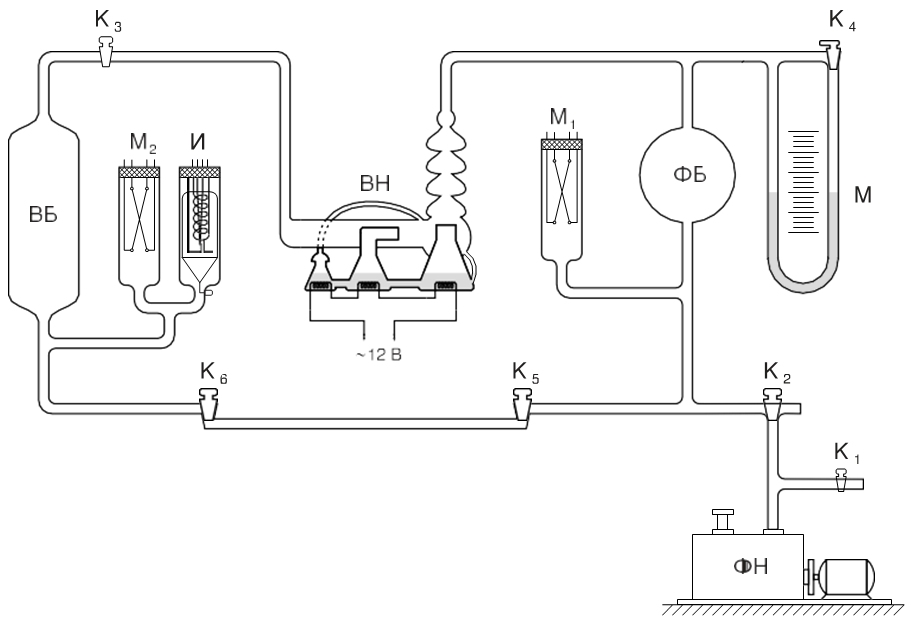
\includegraphics[scale = 0.5]{./images/stand.png}
	\caption{Схема установки}
	\label{fig:stand}
\end{figure}

установка включает в себя краны $K_1, \dots, K_6$, форвакуумный баллон, высоковакуумный диффузионный насос, высоковакуумный баллон, разного вида манометры, форвакуумный насос.

Принцип действия форвакуумного ротационного насоса представлен на следующей схеме:

\begin{figure}[H]
	\centering
	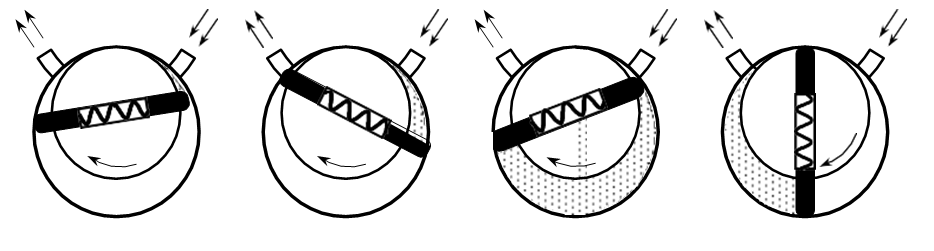
\includegraphics[scale = 0.5]{./images/RotScheme.png}
	\caption{}
\end{figure}
После включения этого насоса нужно дождаться, пока он откачает собственный объем, а только потом подключать его к установке.

Диффузионный насос работает по следующему принципу:

\begin{figure}[H]
	\centering
	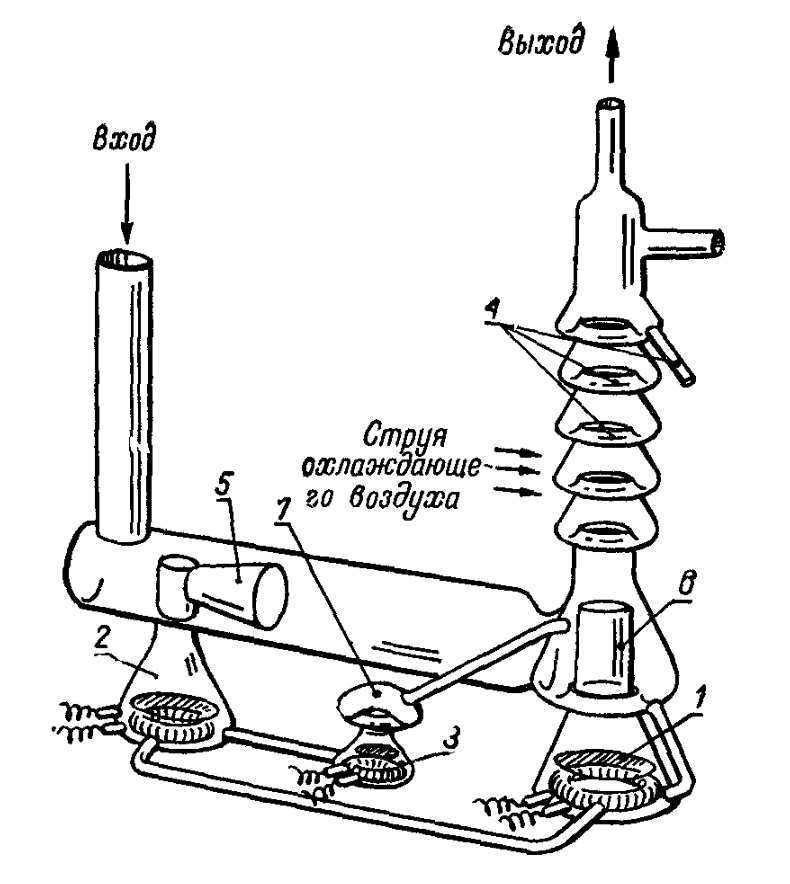
\includegraphics[scale = 0.5]{./images/Difus.png}
	\caption{Диффузионный насос}
\end{figure}
Молекулы газа, попадая в поток масляных паров, увлекаются им и не могут попасть обратно. Этот эффект оказывает сильное откачивающее воздействие на газ в сосуде. Диффузионный насос работает более эффективно, когда длина свободного пробега молекул примерно равна зазору между трубкой и соплом (5).

В установке используются несколько видов манометров. U-образный не представляет никакого интереса, поэтому перейдем сразу к описанию термопарного манометра:

\begin{figure}[H]
	\centering
	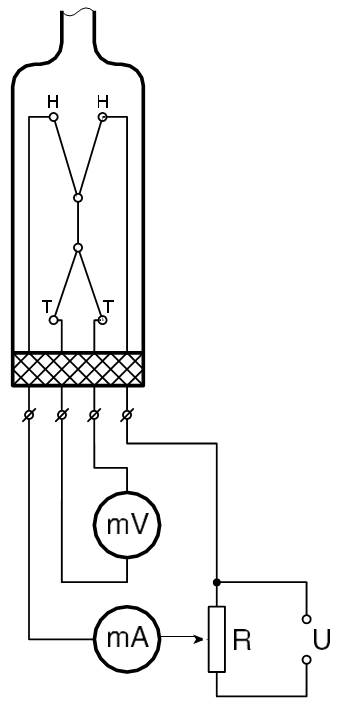
\includegraphics[scale = 0.3]{./images/ThermMan.png}
	\caption{Термопарный манометр}
\end{figure}
Через нить накаливания пропускается ток, регулируемый потенциометром R, а с помощью термопары измеряется нагрев нити, который зависит в том числе от давления газа. Характеристику данной термопары можно увидеть на графике:

\begin{figure}[H]
	\centering
	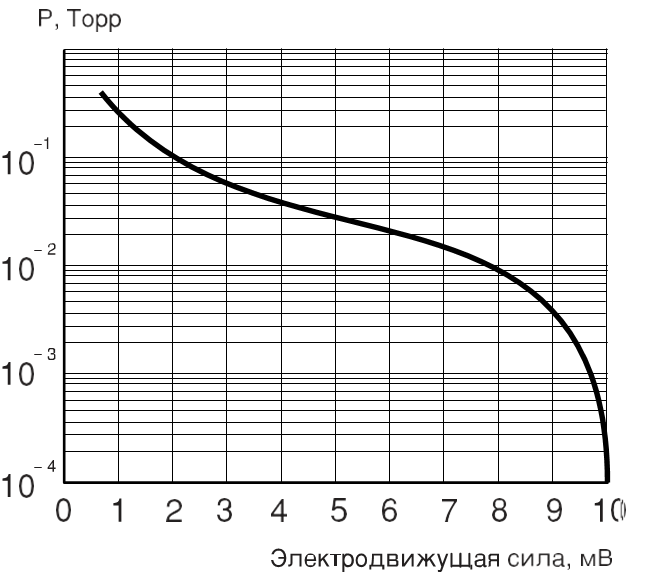
\includegraphics[scale = 0.3]{./images/TChar.png}
	\caption{{Характеристика термопары}}
\end{figure}

Рассмотрим принцип работы ионизационного манометра:

\begin{figure}[H]
	\centering
	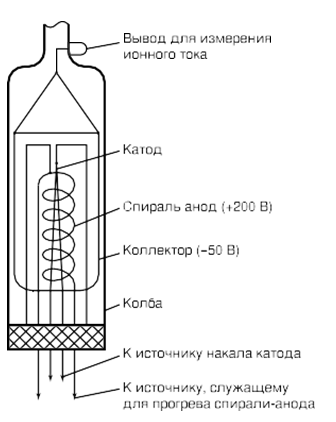
\includegraphics[scale = 0.5]{./images/IonLamp.png}
	\caption{{Ионизационный манометр}}
\end{figure}
Электроны, выпускаемые катодом, прежде чем осесть на аноде успевают ионизировать воздух в колбе. Затем, ионы воздуха оседают на коллекторе. Измеряя ток, образованный ионизированным воздухом, можно определить его давление.

\section{Приборы и материалы}

В работе используются:

\begin{itemize}
	\item Вакуумная установка;
	\item Масляный манометр;
	\item Термопарный манометр;
	\item Ионизационный манометр.
\end{itemize}

\section{Обработка результатов}



\section{Вывод}



\end{document}